%%%%%%%%%%%%%%%%%%%%%%%%%%%%%%%%%%%%%%%%%
% University Assignment Title Page 
% LaTeX Template
% Version 1.0 (27/12/12)
%
% This template has been downloaded from:
% http://www.LaTeXTemplates.com
%
% Original author:
% WikiBooks (http://en.wikibooks.org/wiki/LaTeX/Title_Creation)
%
% License:
% CC BY-NC-SA 3.0 (http://creativecommons.org/licenses/by-nc-sa/3.0/)
% 
% Instructions for using this template:
% This title page is capable of being compiled as is. This is not useful for 
% including it in another document. To do this, you have two options: 
%
% 1) Copy/paste everything between \begin{document} and \end{document} 
% starting at \begin{titlepage} and paste this into another LaTeX file where you 
% want your title page.
% OR
% 2) Remove everything outside the \begin{titlepage} and \end{titlepage} and 
% move this file to the same directory as the LaTeX file you wish to add it to. 
% Then add \input{./title_page_1.tex} to your LaTeX file where you want your
% title page.
%
%%%%%%%%%%%%%%%%%%%%%%%%%%%%%%%%%%%%%%%%%
%\title{Title page with logo}
%----------------------------------------------------------------------------------------
%	PACKAGES AND OTHER DOCUMENT CONFIGURATIONS
%----------------------------------------------------------------------------------------

\documentclass[12pt]{article}
\usepackage[english]{babel}
\usepackage[utf8x]{inputenc}
\usepackage{amsmath}
\usepackage{graphicx}
\usepackage[colorinlistoftodos]{todonotes}
\usepackage{float}
\usepackage{listings}
\lstset{
    language=R,
    basicstyle=\ttfamily
}

\begin{document}
\bibliographystyle{unsrtdin}

\begin{titlepage}

\newcommand{\HRule}{\rule{\linewidth}{0.5mm}} % Defines a new command for the horizontal lines, change thickness here

\center % Center everything on the page
 
%----------------------------------------------------------------------------------------
%	HEADING SECTIONS
%----------------------------------------------------------------------------------------

\textsc{\LARGE Humboldt University of Berlin }\\[0.3cm] % Name of your university/college
\textsc{\LARGE Institute of Economics  }\\[0.3cm]
\textsc{\Large Applied Predictive Analytics}\\[0.5cm] % Major heading such as course name
 % Minor heading such as course title

%----------------------------------------------------------------------------------------
%	TITLE SECTION
%----------------------------------------------------------------------------------------

\HRule \\[0.4cm]
{ \huge \bfseries Data Mining Cup 2015:\\[0.5cm] Basket Value Prediction}\\[0.03cm] % Title of your document
\HRule \\[1.5cm]

 
%----------------------------------------------------------------------------------------
%	AUTHOR SECTION
%----------------------------------------------------------------------------------------


\begin{table}[H]
\begin{center}
\begin{tabular}{lcr}
\emph{Submitted By:} & & \emph{Submitted To:} \\
Elisabeth Bommes & & Prof. Dr. Stefan\\
Sophie Burgard &  & Lessmann\\
Ringolf Thomschke\\ % Your name
\end{tabular}
\end{center}
\end{table}


% If you don't want a supervisor, uncomment the two lines below and remove the section above
%\Large \emph{Author:}\\
%John \textsc{Smith}\\[3cm] % Your name

%----------------------------------------------------------------------------------------
%	DATE SECTION
%----------------------------------------------------------------------------------------

{\large Summer term 2015 }\\[1cm] % Date, change the \today to a set date if you want to be precise

%----------------------------------------------------------------------------------------
%	LOGO SECTION
%----------------------------------------------------------------------------------------


\includegraphics{husiegel_sw_op.eps}\\[1cm] % Include a department/university logo - this will require the graphicx package
 
%----------------------------------------------------------------------------------------

\vfill % Fill the rest of the page with whitespace

\end{titlepage}

\tableofcontents
\newpage

\section{Introduction and Task Description}

For the 2015 Data Mining Cup, prudsys AG provided customer data from an online shop. From this data, the contestants had to predict the propensity of customers to redeem a coupon and the customers' basket value. After the release of the training and test data, the challenge was to create and submit predictions on the test data within six weeks. We divided the challenge into several different tasks which up to four team members were assigned to. In this report, we will describe the prediction of the basket value variable.\\ 

\section{Data Description}

The data set consisted of 6053 instances for which 33 variables were given. The distribution of the target variable basket value turned out to be highly right-skewed with a very large range  of over 135000 and showed over 237 of strong extremes (by definition in the boxplot concept). Furthermore, it showed significant peaks at lower levels which, however, remained undescribed in our further analysis. Finding an appropriate algorithm to detect outliers in the basket value variable, was another important task. This will also not be covered by this report as it was assigned to other team members.  The idea is to replace outliers by the customer's mean basket value or, if not available, by the overall mean. In our analysis, we decided to use a rather arbitrary upper fence of 700 for outliers which had been set by the data preparation group. based on the definition of strong extremes in the boxplot and a look at the histogram.

\begin{figure}[H]
\centering
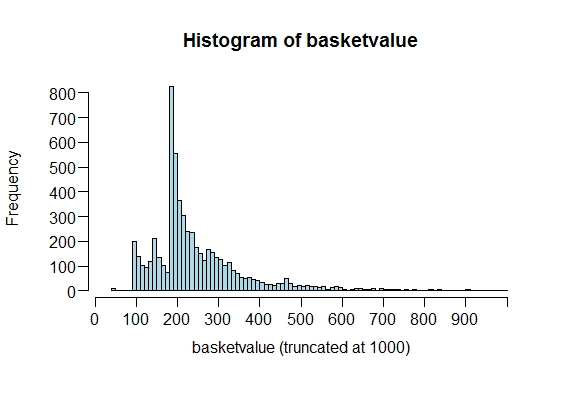
\includegraphics[width=0.83\textwidth]{histbasket.jpeg}
\caption{Distribution of the basket value variable}
\end{figure}

\section{Competition Outcomes}

\subsection{Base Model Selection}

In order to create a library of base classifiers, we used several learning methods in \texttt{R} such as random forests, support vector machines or gradient boosting machines. We estimated a total of 16 different base classifiers on the data set which, after some thoughtful variable building, consisted of 100 variables for each observation. The choice of the specific models is orientated at Delagado (2014), stating that various kinds of random forest models usually perform best, followed by some support vector machines.\cite{Fernandez-Delgado2014}The models were trained on randomly chosen 80 \% of the given data. The remaining 20 \% served as hold-out sample to test, validate and compare the base classifiers on unseen data.

The model estimation and parameter tuning was performed using the \texttt{R}-package \texttt{caret} (short for \textit{C}lassification \textit{a}nd \textit{re}gression \textit{t}raining). A five-fold cross-validation was implemented to determine the model parameters. The models were trained to minimize the following by the competition given assessment criterion on the data:

\[AC = \sum_{i=1}^n \frac{|basketValue_{i} - basketValuePrediction_{i}|}{\frac{1}{n} \sum_{j=1}^n basketValue_{i}}\]

The respective value of the above standing criterion for different base classifiers is listed in Table 1, "Model" refers hereby to the corresponding model name in the \texttt{R}-package \texttt{caret}.

\begin{table}
\centering
\begin{tabular}{l|cc}
\hline
\hline
Model & AC Holdout- &AC Test-Set \\
& Sample (n=1210)  &  (n=669) \\\hline
UserID-Model & 2486 & 1167 \\
\texttt{cubist} & 3355 & 1741\\
Ensemble & 3390 & 1766 \\
\texttt{parRF} & 3466 & 1817 \\
\texttt{RRF} & 3467 & 1816\\
\texttt{RRFglobal} & 3467 & 1816\\
\texttt{rf} & 3468 & 1815\\
\texttt{qrf} & 3472 & 1817\\
\texttt{ctree} & 3475 & 1816\\
\texttt{cforest} & 3485 & 1824\\
\texttt{gbm }& 3469 & 1825\\
\texttt{blackboost} & 3506 & 1830\\
\texttt{mlp} & 3742 & 1971\\
\texttt{svmRadialCost} & 3786 & 1995\\
\texttt{svmRadial} & 3742 & 1995\\
\texttt{mlpWeightDecay} & 3832 & 2020\\
\hline
\hline
\end{tabular}
\caption{Evaluation of Base Classifiers (without obvious misclassifiers (AC over 100 000)}
\end{table}

Most of the models aim towards a relatively similiar prediction power. But the smallest prediction error was made by a more insightful model which predicted the basket value variable by taking the mean of previous basket values for known customers and predicting for unknown customers over some random forest model. 
We suspect the inferiority of the machine learning under a much more simpler model being caused by the drawing mechanism of the 20\% hold-out sample and will investigate this issue in a later part of this report.

%Moreover, calculation of the models turned out to be relatively calculus intensive, taking up to 24 hours to obtain estimates for all mentioned models. We will approach the issue of parallelization in the following section. \\


\subsection{Ensemble Selection}

To combine the various model predictions to one single value for each data point, we used the technique of ensemble selection.\cite{Caruana04} Ensemble selection aims for a superior prediction power by determining a weighted mean of the predicted values made by different base classifiers. Idea behind that is to overcome shortcomings of various model types. For the given data set the algorithm determined weights according to Table 2. The overall prediction error for the ensemble with the given weights on the hold-out sample is 3390, therefore performing second best after the best base classifier (\texttt{cubist} 3355).

\begin{table}
\centering
\begin{tabular}{l|cccccc}
\hline
\hline
model &\texttt{qrf} & \texttt{cubist} & \texttt{parRF} & \texttt{rf} & \texttt{RRF} & \texttt{blackboost} \\ \hline
weight &0.05 & 0.6 & 0.2 & 0.0985 & 0.05 & 0.0015\\
\hline
\hline
\end{tabular}
\caption{Models Within The Ensemble And Corresponding Weights}
\end{table}


\section{Post-Processing}

In the following section we are going to investigate the reasons for the inferior performance of the machine learning techniques in estimating the basket value variable via a simulation study. In line with the simulation stood the focus on the post editing of the programming code, especially parallelization issues to shorten the needed calculation time.

One reason for the bad performance of any machine learning technique we suspect in the mechanism how the separation between holdout- and training-sample was made: The 20\% test set was randomly chosen in the process of predicting the first of the binary coupon variables via an in the \texttt{caret}-package included function \texttt{createDataPartition} and using the same sample for all other target variables. By using this function the sampling mechanism aims to maintain the distribution of the target variable, in this case of one of the coupons. We suspect that this way of sampling leads to an insufficient distribution of the basket value variable in the hold-out sample and therefore yielding deficient prediction results.

\begin{figure}[H]
\centering
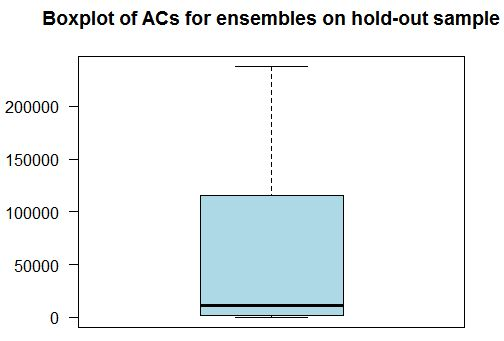
\includegraphics[width=0.83\textwidth]{boxplotACES.jpg}
\caption{Boxplot of the assessment criteria for the 98 ensembles on hold-out sample}
\end{figure}

By taking a look at the boxplot (Fig. 2) and the summary statistics (Tab. 3) for the 98 ensembles' assessment criteria, we notice the very large range. Also, the median is higher than any AC from the competition. One can conclude from these results that partitioning the data with respect to the target variables distribution does not, in general, lead to lower results for the assessment criterion. Presumably, this is due to the fact that the DMC metric allocates a very high penalty to mispredicted outliers. The number of outliers in the hold-out sample can increase the AC severely as the difference between observation and prediction is squared. However, as mentioned above, the target variable shows a large range of strong extremes and, therefore, the machine learning techniques seem unable to prevent stark mispredictions.

\begin{table}
\centering
\begin{tabular}{|c|c|c|c|c|c|}
\hline
\hline
mean & median & sd & min & max & range\\
\hline
56153 & 11033 & 69616 & 404 & 237538 & 237134\\
\hline
\hline
\end{tabular}
\caption{Summary statistics for assessment criteria of the 98 ensembles on hold-out sample}
\end{table}

Indeed, the simulation study produced a high number of ensembles which are inferior to those built during the competition. Yet, we were now able to choose from 98 samples of base classifier and ensembles. The minimal ACs of these sample were all lower than the ones collected during the competition (Tab. 4). This shows the advantage of having a large amount of base classifiers that were trained on differently partitioned data sets. One can decrease the probability of having a highly skewed hold-out sample by simply creating more randomly partitioned data sets on which the base classifiers are trained.

\begin{table}
\centering
\begin{tabular}{l|cc}
\hline
\hline
Model & Competition AC & Simulation study AC\\
\hline
Ensemble 			& 3390 		& 404\\
\texttt{RRF} 		& 3467 		& 485\\
\texttt{RRFglobal} 	& 3467 		& 700\\
\texttt{rf} 		& 3468 		& 660\\
\texttt{qrf} 		& 3472 		& 755\\
\texttt{ctree} 		& 3475 		& 670\\
\texttt{cforest} 	& 3485 		& 957\\
\texttt{gbm }		& 3469 		& 1892\\
\texttt{blackboost} & 3506 		& 919\\
\texttt{mlp} 		& 3742 		& 836\\
\texttt{svmRadialCost} & 3786 	& 819\\
\texttt{svmRadial} 	& 3742 		& 820\\
\texttt{mlpWeightDecay} & 3832 	& 834\\
\hline
\hline
\end{tabular}
\caption{Comparison of minimal assessment criteria collected in the competition and in the simulation study.}
\end{table}

After the competition was finished, prudsys AG provided target variable values which now enabled us to examine the performance of our ensembles on the validation set. By taking a look on the upper part of Figure 3, we observe that, only two ensemble perform worse than the mean prediction on the validation set. Other observations lie rather symmetrically distributed around the AC mean. Looking at the bottom part of Figure 3, we realize that the ensemble with the lowest score on the hold-out sample has an average performance on the validation set. Other ensemble with slightly higher AC on their hold-out sample show better results on the validation set. Nevertheless, the very low scores on the validation set can be found in the region up to an AC value of 3500 for the hold-out sample. Therefore, to choose an ensemble with good performance on the hold-out sample is still reasonable.\\

\begin{figure}[H]
\centering
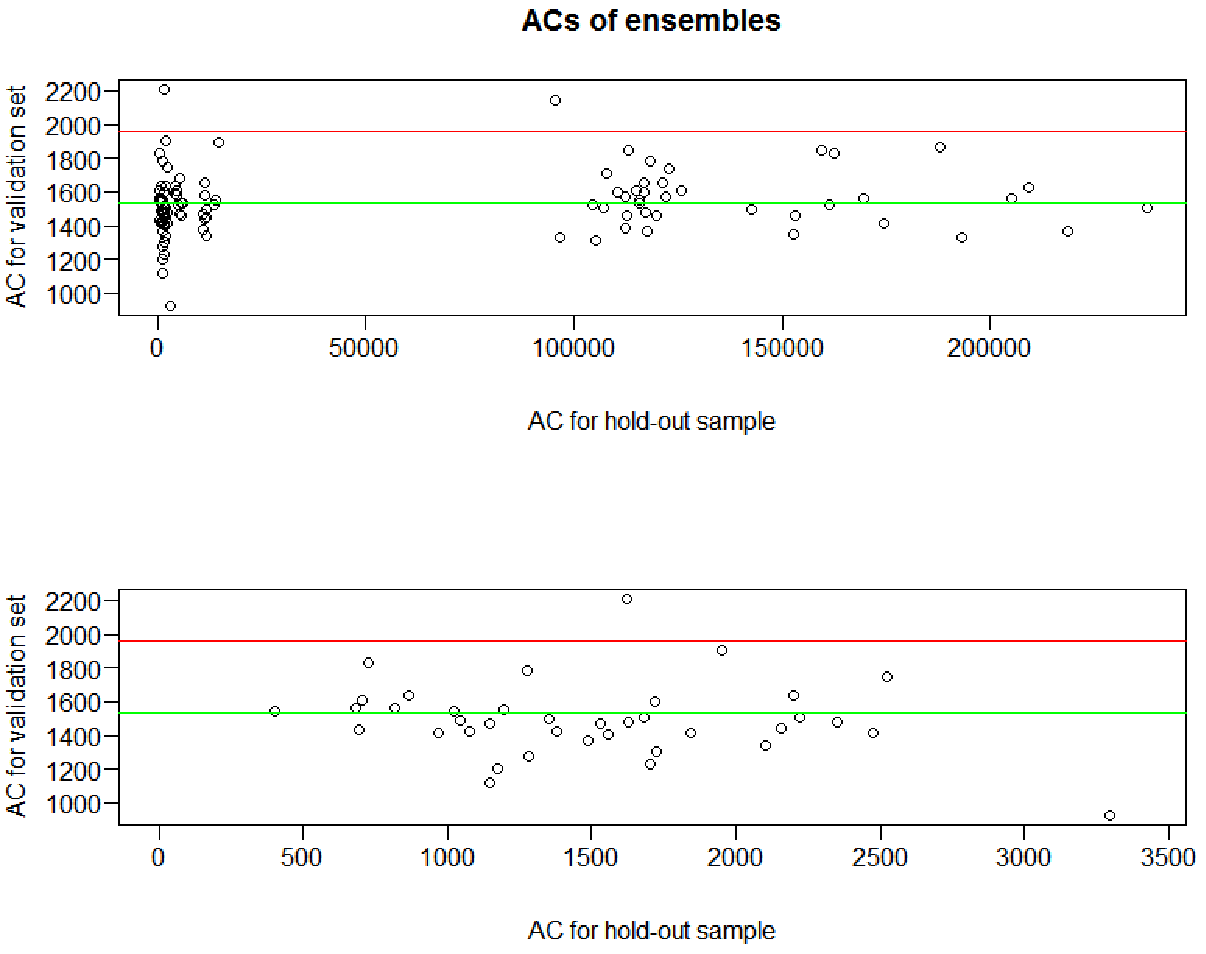
\includegraphics[width=0.83\textwidth]{ACensemble.pdf}
\caption{Scatterplot of ACs of ensembles for hold-out sample and validation set. (Top) the entire range of ACs for hold-out sample, (bottom) truncated at 3500. Red lines indicate the AC of a mean prediction, green lines indicate the average AC on the validation set.}
\end{figure}

\section{Summary}

By conducting a simulation study for the prediction of basket values with ensemble selection, we gained further insight in the importance of partitioning and outlyingness in the context of machine learning techniques. 

Our first assumption was that the inferiority of machine learning models compared to the straight-forward customer mean prediction was caused by an undue partitioning of the data which did not take the target variable distribution into account. This assumption could not be verified most likely because of the very large range of outliers. However, we still consider this technique as the correct approach even if it cannot be substantiated by our result.

More importantly, with our simulation study we produced superior results for the assessment criteria for all base classifiers and in the ensemble selection. This was possible due to the mere amount of models we simulated on different randomly partitioned data sets. By using differently partitioned data sets for training and testing we decreased the probability of drawing highly skewed hold-out samples which, in general, yield bad performance meassures.

A final evaluation on the validation set with observations provided after the competition allowed for further examination of the estimated ensembles.\\

\nocite{Caruana2006}
\nocite{Niculescu-Mizil2009}

\newpage
\appendix
\section{Appendix}
R Code

\begin{itemize}
	\item Data Preparation.R
    \item Model Estimation.R
    \item Prediction Extraction.R
    \item Test Prediction.R
    \item Ensemble Selection.R
    \item Results.R
\end{itemize}

\newpage
\lstinputlisting{Data_Preparation.R}
\newpage
\lstinputlisting{Model_Estimation.R}
\newpage
\lstinputlisting{Prediction_Extraction.R}
\newpage
\lstinputlisting{Test_Prediction.R}
\newpage
\lstinputlisting{Ensemble_Selection.R}
\newpage
\lstinputlisting{Results.R}

\newpage
\bibliography{literature}


\end{document}